\documentclass[tikz,border=8pt]{standalone}
% Shared look for every TikZ diagram. Load with \input{../../tools/tikz-style.tex}
\usepackage[T1]{fontenc}
\usepackage{lmodern}
\renewcommand{\sfdefault}{lmr}  % diagrams use the same serif as the text
\usetikzlibrary{arrows.meta, positioning, shapes.geometric, calc, fit, backgrounds}
\definecolor{cblue}{HTML}{4C78A8}
\definecolor{corange}{HTML}{F58518}
\definecolor{cgreen}{HTML}{54A24B}
\definecolor{cred}{HTML}{E45756}
\definecolor{cpurple}{HTML}{B279A2}
\definecolor{cgrey}{HTML}{6B6B6B}
\tikzset{
  every picture/.style={font=\sffamily, line width=1.2pt},
  box/.style={draw=#1, fill=#1!12, rounded corners=4pt, align=center, inner sep=7pt, minimum height=1.1cm},
  box/.default=cgrey,
  arrow/.style={-{Stealth[length=3mm]}, draw=cgrey, line width=1.4pt},
  title/.style={font=\sffamily\bfseries\Large},
  note/.style={font=\sffamily\small, text=cgrey, align=center},
}
\AtBeginDocument{\hyphenpenalty=10000 \exhyphenpenalty=10000}

\begin{document}
% Section 6: the world database's three tables (row counts from data/world.db) and how they link: city.CountryCode
% and countrylanguage.CountryCode both point to country.Code.
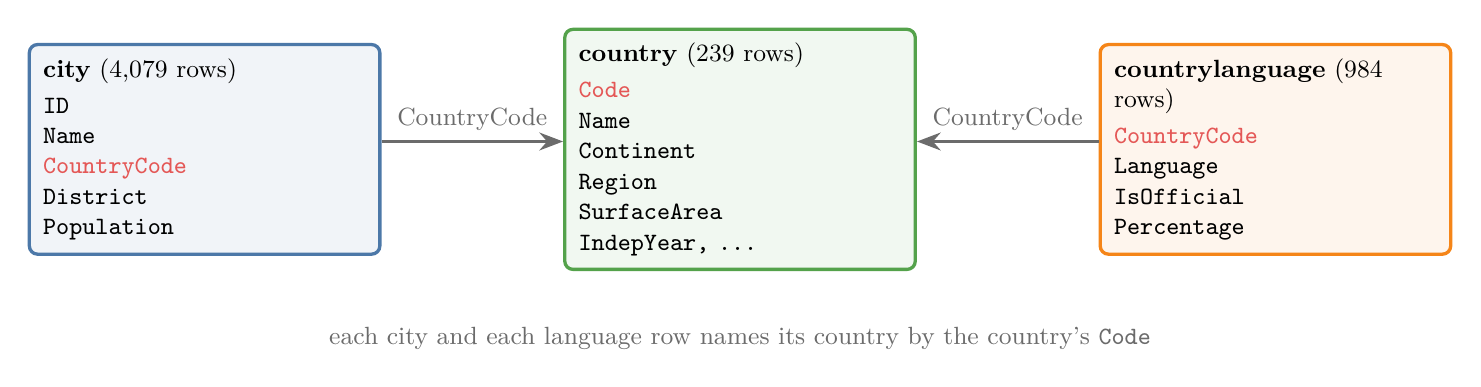
\begin{tikzpicture}[tbl/.style={draw=#1, fill=#1!8, rounded corners=3pt, align=left, inner sep=5pt, font=\ttfamily\small, text width=4.1cm},
  hd/.style={font=\sffamily\bfseries}]
  \node[tbl=cblue] (city) at (0, 0) {\textsf{\textbf{city}} \textsf{(4,079 rows)}\\[2pt]ID\\Name\\\textcolor{cred}{CountryCode}\\District\\Population};
  \node[tbl=cgreen] (country) at (6.8, 0) {\textsf{\textbf{country}} \textsf{(239 rows)}\\[2pt]\textcolor{cred}{Code}\\Name\\Continent\\Region\\SurfaceArea\\IndepYear, \dots};
  \node[tbl=corange] (lang) at (13.6, 0) {\textsf{\textbf{countrylanguage}} \textsf{(984 rows)}\\[2pt]\textcolor{cred}{CountryCode}\\Language\\IsOfficial\\Percentage};
  \draw[arrow, draw=cgrey] ([yshift=0.1cm]city.east) -- ([yshift=0.1cm]country.west) node[midway, above, note] {CountryCode};
  \draw[arrow, draw=cgrey] ([yshift=0.1cm]lang.west) -- ([yshift=0.1cm]country.east) node[midway, above, note] {CountryCode};
  \node[note] at (6.8, -2.4) {each city and each language row names its country by the country's \texttt{Code}};
\end{tikzpicture}
\end{document}
